\begin{center}
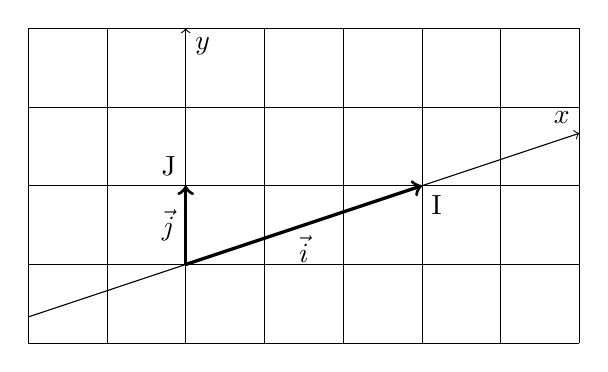
\begin{tikzpicture}
	% Dimensions du repere
	\def\xmin{-2} 
	\def\xmax{5} 
	\def\ymin{-1} 
	\def\ymax{3}
	% Grille
	\draw [very thin] (\xmin,\ymin) grid (\xmax,\ymax); 
	% Annotations axes et unites
	\draw [->] (-2,-2/3)--(5,5/3) node[above left]  {$x$};
	\draw [->] (0,\ymin)--(0,\ymax) node[below right] {$y$};
	\draw [->,very thick] (0,0)-- node[below] {$\vec{i}$} (3,1);
	\draw [->,very thick] (0,0)-- node[left] {$\vec{j}$} (0,1);
	\draw (3,1) node[below right] {I};
	\draw (0,1) node[above left] {J};
	% Clip pour que les figures ne sortent pas du cadre
	\clip (\xmin,\ymin) rectangle (\xmax,\ymax); 
\end{tikzpicture}
\end{center}
